\documentclass[12pt]{article}
\usepackage[hmargin=3.4cm,a4paper]{geometry}
\usepackage{polyglossia}
\setdefaultlanguage{french}
\frenchspacing
\usepackage{amssymb,amsfonts}
\usepackage{mathtools}
\usepackage{hyperref}
\usepackage[dvipsnames]{xcolor}
\usepackage{graphicx}
\usepackage{standalone}
\usepackage{import}
\usepackage[thref,hyperref,amsmath]{ntheorem}
\usepackage{titling}
\usepackage{tikz}
\usepackage{listings}

\lstset{language=python,
	basicstyle=\ttfamily,
	keywordstyle=\color{OliveGreen},
    columns=fixed}

%%%%% Environnements exercice et correction %%%%%
\theoremstyle{break}
\theoremheaderfont{\normalfont\bfseries}
\theorembodyfont{\normalfont}
\newtheorem{cor}{Correction de l'exercice}
\theoremheaderfont{\normalfont\bfseries}
\newtheorem{exo}{Exercice}

%%%%% Ensembles usuels %%%%%
\newcommand{\NN}{\mathbb N}
\newcommand{\ZZ}{\mathbb Z}
\newcommand{\QQ}{\mathbb Q}
\newcommand{\PP}{\mathbb P}
\newcommand{\EE}{\mathbb E}
\newcommand{\VV}{\mathbb V}
\newcommand{\RR}{\mathbb R}
\newcommand{\CC}{\mathbb C}


\pretitle{\begin{center}\LARGE\scshape}
\title{Tremplin: Exercices}
\posttitle{\end{center}}

\preauthor{}
\author{}
\postauthor{}

\begin{document}

\maketitle

\textit{Recueil d'exercices destinés aux séances de l'association Tremplin au lycée Marcel Pagnol d'Athis-Mons.}


\section*{Énoncés}

\begin{exo}
On veut acheter plusieurs exemplaires de deux produits 1 et 2. On dépense 40€ en achetant 3 unités du bien 1 et 5 du bien 2.

Quels sont les prix (possibles) des produits 1 et 2 ?

On suppose désormais qu'acheter un de chaque coûte 10€. Déterminer les prix des deux produits.
\end{exo}


\begin{exo}[Algorithmes de tri, partie 1]
Soit $n$ un nombre entier positif. Soit une liste de $n$ éléments $a_1,\ldots,a_n$. On suppose que l'on peut les comparer les uns aux autres, et que l'on veut les trier dans l'ordre croissant. Comment faire ?

\textit{Indication: Comment faire pour choisir le plus petit élément de la liste ?}

Combien d'opérations sont effectuées pour trier une liste de $n$ nombres ?
\end{exo}


\begin{exo}[Tasse de café et tasse de lait]
On a deux tasses identiques, l'une avec du café, l'autre avec du lait. On prend une cuillère, et on prélève délicatement du lait dans le la tasse de lait. On verse le contenu dans la tasse de café, et on mélange bien. On prélève maintenant une cuillère du mélange qu'on verse dans la tasse de lait, et on mélange bien.

\begin{figure}[!ht]
	\centering
	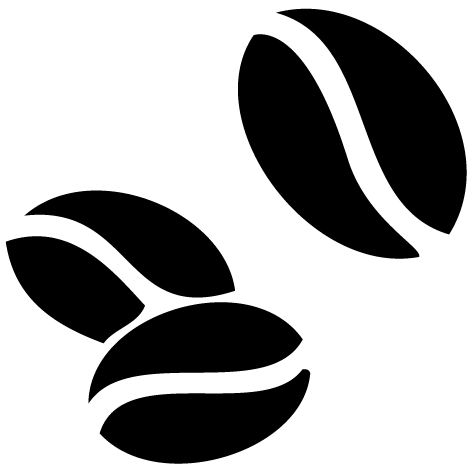
\includegraphics[width=0.2\textwidth]{images/grainCafe.png}
    
\includegraphics[width=0.3\textwidth]{images/LogoJava.png}
    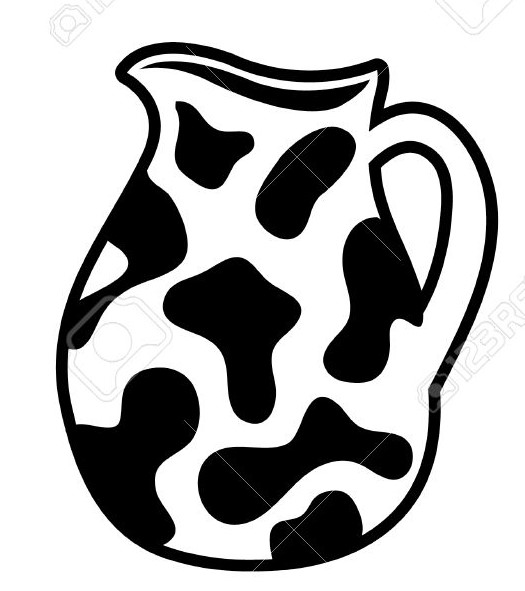
\includegraphics[width=0.2\textwidth]{images/potAlait.jpg}
\end{figure}

Y a-t-il plus de lait dans la tasse de café ou de café dans la tasse de lait ?

\end{exo}


\begin{exo}[Énigmes des cavaliers d'Al-Adli]
Prenons un échiquier de 9 cases avec 1 cavalier blanc et 1 noir, sur deux cases opposées.

Combien faut-il de coup pour que le cavalier blanc se retrouve sur la case initiale du noir et vice versa ?

Sur le même échiquier, prenons maintenant 2 cavaliers blancs, placés dans les coins supérieurs, et 2 noirs, dans les coins inférieurs.

Combien faut-il désormais de coups pour échanger les cavaliers ?

Avec maintenant 3 cavaliers de part en d'autre, combien faut-il de coups ? \textit{Émettez une conjecture avant de résoudre le problème.}


\begin{figure}[h!]
	\centering
	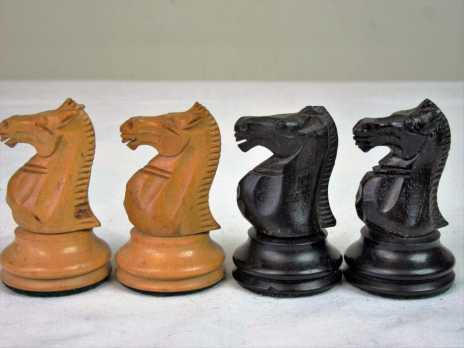
\includegraphics[width=0.35\textwidth]{images/4Cavaliers.jpg}
\end{figure}
\end{exo}


\begin{exo}[Celui qui lit dans les cartes...]
Deux magiciens vous ont préparé un petit tour de magie :

Le premier sort de la pièce en fermant bien la porte.

Le second bat un paquet de 52 cartes (sans joker). Ils vous en fait piocher 5 au hasard. Il en prend une, la montre à tout le monde et vous la confie en vous demandant de la tenir secrète.

Ils dispose les 4 autres cartes sur la table et fait entrer son collègue.

Son collègue entre en disant : << Je sais quel carte vous cachez ! C'est facile, c'est le ... >>. Surprise : il a raison !

Comment a-t-il fait pour deviner la carte que vous aviez si soigneusement dissimulée ?


\begin{figure}[h!]
	\centering
	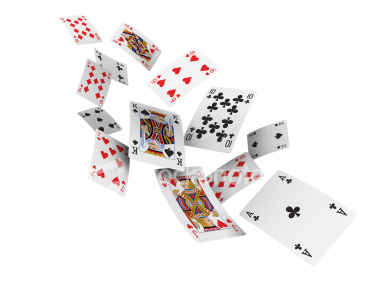
\includegraphics[width=0.35\textwidth]{images/Cartes.jpeg}
\end{figure}
\end{exo}


\begin{exo}[La prise de la Bastille... c'était quel jour ?]
La prise de la Bastille, la prise de la Bastille... c'était quel jour de la semaine déjà ?

\begin{figure}[h!]
	\centering
	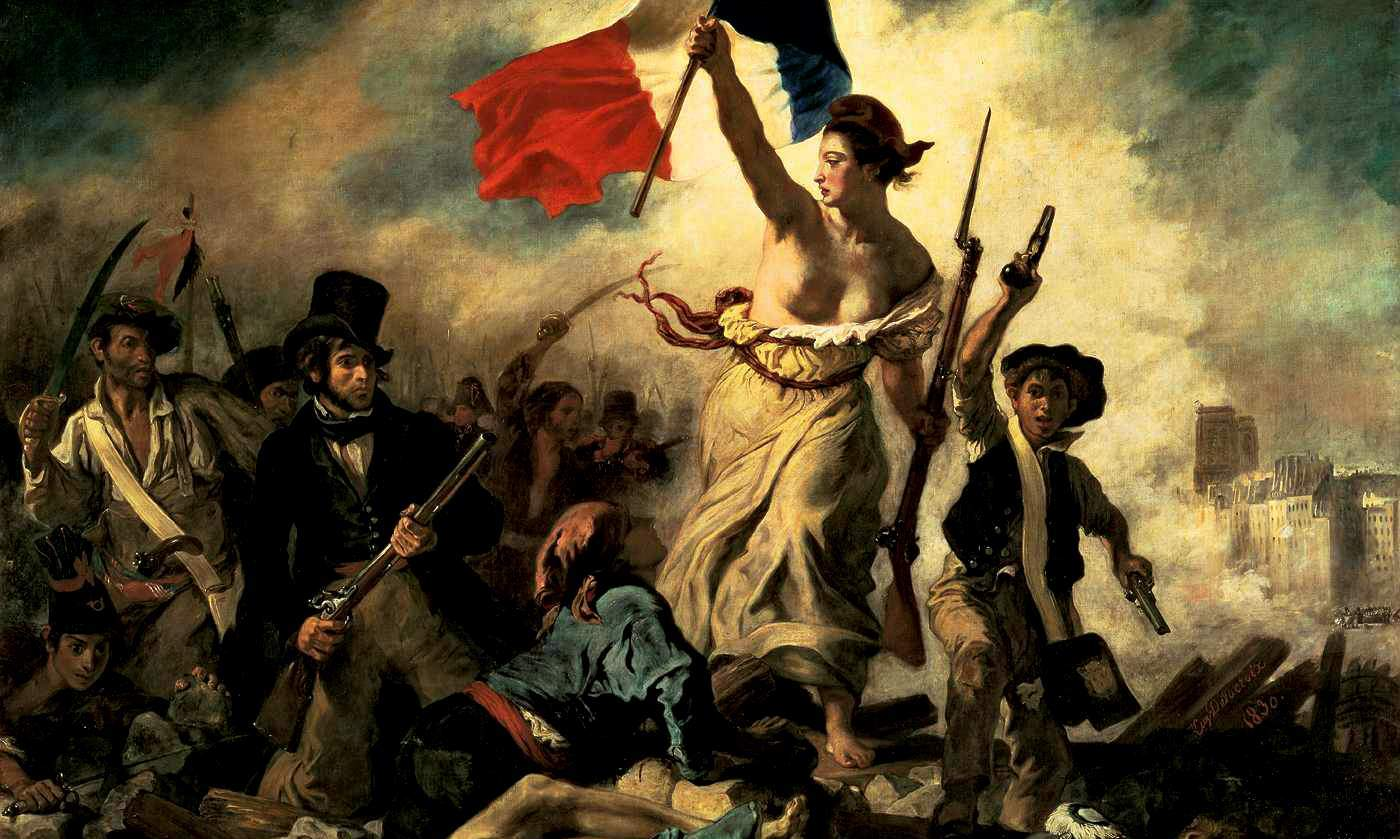
\includegraphics[width=0.445\textwidth]{images/MarianneGuidantLePeuple.jpg}
    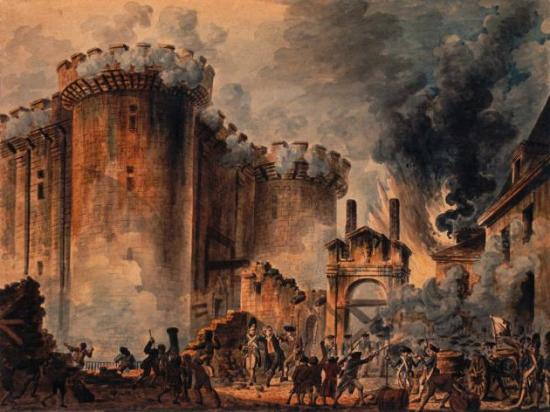
\includegraphics[width=0.35\textwidth]{images/PriseDeLaBastille.jpg}
\end{figure}
\end{exo}


\begin{exo}[Paradoxe des anniversaires]
Dans votre classe, n'y a-t-il pas deux personnes qui ont leurs anniversaires le même jour ? Étrange coïncidence ? Combien êtes-vous dans votre classe ? À votre avis, combien de personnes minimum faut-il pour qu'il y ait plus d'une chance sur deux que deux anniversaires au moins tombent à la même date ?

\begin{figure}[h!]
	\centering
	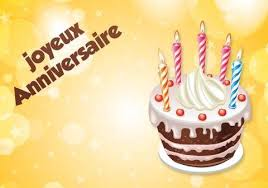
\includegraphics[width=0.3\textwidth]{images/AnniversaireGateau.jpg}
    
\includegraphics[width=0.35\textwidth]{images/ReflexionAnniversaire.jpg}
\end{figure}
\end{exo}


\begin{exo}[Tétraèdre à couper]
On prend un tétraèdre régulier. Il est facile de le couper en deux parties de même volume, voire de même aire latérale. Mais comment, en un seul coup de couteau, le couper en deux parties parfaitement superposables ?

\begin{figure}[h!]
	\centering
    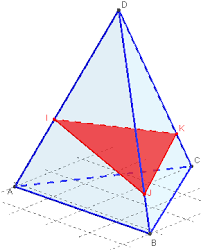
\includegraphics[width=0.26\textwidth]{images/CoupeTetraedre.png}
\end{figure}
\end{exo}


\begin{exo}[Marche aléatoire]
Jean-Michel est saoul et revient du bistrot. À chaque pas, il a une chance sur deux d'aller vers l'avant ou vers l'arrière.
\begin{enumerate}
\item Jean-Michel peut-il espérer rentrer chez lui ?
\item Quelle est, en moyenne, la distance dont Jean-Michel peut espérer s'éloigner de son point de départ au bout de $t$ pas ?
\end{enumerate}

\begin{figure}[!ht]
\centering
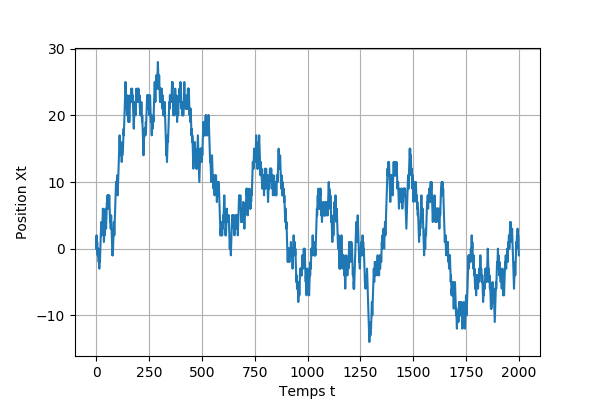
\includegraphics[width=0.6\textwidth]{images/marcheJM.png}
\end{figure}

\end{exo}


\begin{exo}[Heures et équerres]
Prenez une horloge, avec ses aiguilles qui tournent en tout sens. À 9h00 et 3h00, la grande et la petite aiguilles sont précisément perpendiculaires, mais quand cela se produit-il d'autre dans la journée ? Et combien de fois ?

Une fois parvenu au résultat, vous pouvez recommencer avec un angle quelconque entre les aiguilles.

\begin{figure}[h!]
	\centering
    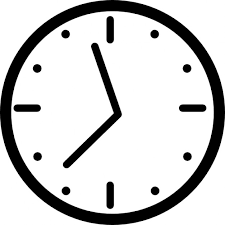
\includegraphics[width=0.15\textwidth]{images/horloge.png}
\end{figure}
\end{exo}


\begin{exo}[Pile de crêpes]
Germain fait des crêpes, beaucoup de crêpes. Il les empile à la va vite, sans se préoccuper de leurs tailles. Néanmoins, la pile est tout sauf présentable : les crêpes glissent les unes sur les autres en un tas informe. Il vous faut donc les ranger, de la plus grande en bas à la plus petit en haut. Pour ce faire, vous ne disposer que d'une seule action : vous glisser votre spatule quelque part entre deux crêpes, et vous retourner d'un bloc le dessus de la pile.

Comment faire ? Combien de coups au minimum sont nécessaires pour ranger une pile de $72$ crêpes ?

\begin{figure}[h!]
	\centering
    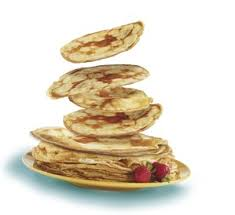
\includegraphics[width=0.3\textwidth]{images/PileDeCrepes.jpg}
\end{figure}
\end{exo}


\begin{exo}[Tours de Hanoï]
On dispose devant nous trois bâtons. Sur celui de gauche sont enfilés 8 disques percés, posés les uns sur les autres, du plus gros (en bas) au plus petit. On veut déplacer cette "tour" sur le bâtons de droite, un disque par un disque, sans jamais qu'un gros disque se retrouve sur un plus petit.

Comment faire ? Combien de coups au minimum sont nécessaires ?

\begin{figure}[h!]
	\centering
    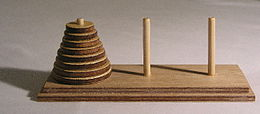
\includegraphics[width=0.5\textwidth]{images/TourDeHanoi.jpeg}
\end{figure}
\end{exo}


\begin{exo}[Deux portes]
Devant vous, il y a deux portes : l'une mène chez le Père Noël et l'autre chez le Père Fouettard. Devant une porte se trouvent Suzie, et devant l'autre Germain : l'un dit toujours la vérité et l'autre est un éternel menteur, mais vous ignorez qui est qui... Vous ne pouvez poser qu'une seule question et ouvrir qu'une seule porte : que faire ?

\begin{figure}[h!]
	\centering
    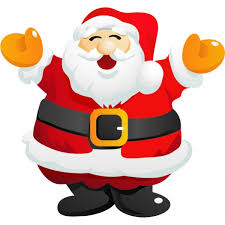
\includegraphics[width=0.25\textwidth]{images/PereNoel.jpg}
    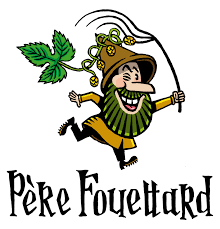
\includegraphics[width=0.25\textwidth]{images/PereFouettard.png}
\end{figure}
\end{exo}


\begin{exo}[Théorie des jeux : Coopération \& Trahison]
Vous jouez avec votre voisin à un jeu d'argent. Les règles sont simples : à chaque tour, chacun peut choisir de miser 1€ ou de le garder pour lui. Si les deux joueurs misent, ils gagnent tous les deux 3€. Si l'un des deux mise mais pas l'autre, celui qui n'a pas misé emporte 5€ alors que l'autre n'a rien. Si personne ne mise, chacun repart avec 1€. On joue 15 tours, puis on fait les comptes.

Proposez chacun une stratégie (c'est-à-dire un ensemble de règles régissant votre comportement), et mettez-là en pratique par binôme, puis changer de binôme jusqu'à avoir affronté tous vos camarades. Notez au fur et à mesure les résultats sur les feuilles dédiées.

\begin{figure}[h!]
	\centering
    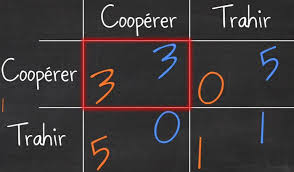
\includegraphics[width=0.4\textwidth]{images/CooperationTrahison.jpg}
\end{figure}
\end{exo}


\begin{exo}[Chat échaudé craint l'eau froide]
On vous a toujours dit que l'eau chaude est moins dense que l'eau froide, plus dilatée ? Mais en êtes-vous sûr ? Proposez plusieurs expérience tendant à prouver que l'eau chaude est moins dense que l'eau froide (ou le contraire).

\begin{figure}[h!]
	\centering
    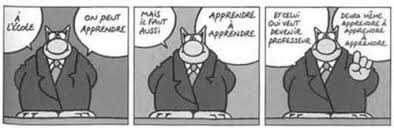
\includegraphics[width=0.75\textwidth]{images/LeChat1.jpg}
\end{figure}

\begin{figure}[h!]
	\centering
    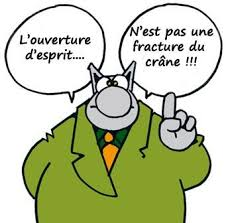
\includegraphics[width=0.29\textwidth]{images/LeChat2.jpg}
    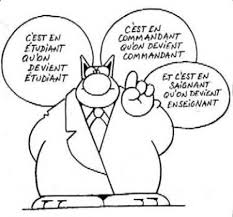
\includegraphics[width=0.29\textwidth]{images/LeChat3.jpg}
\end{figure}
\end{exo}


\begin{exo}[Pièce qui roule...]
On vous donne deux pièces de monnaie (temporairement). Vous faites rouler l'une sur l'autre, tranche contre tranche. Lorsque la pièce extérieure est revenue à son point de départ, combien de tour sur elle-même a-t-elle fait ?

\begin{figure}[h!]
	\centering
    
\includegraphics[width=0.4\textwidth]{images/PieceDeMonnaie.jpg}
\end{figure}
\end{exo}


\begin{exo}[Est-ce que la taille compte vraiment ?]
La Terre est bien plus grande qu'un ballon de foot, non ? On prend un ballon de foot et la Terre, et on augmente leur deux rayons d'un mètre. Du ballon et de la Terre, laquelle des deux circonférences augmente le plus ?

\begin{figure}[h!]
	\centering
    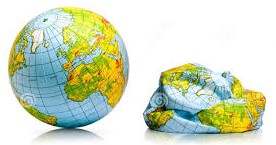
\includegraphics[width=0.4\textwidth]{images/Terre.jpg}
    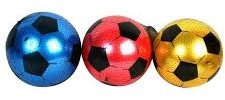
\includegraphics[width=0.4\textwidth]{images/BallonFoot.jpg}
\end{figure}
\end{exo}


\begin{exo}[Les couleurs qui dansent]
Le lait n'est pas que pour les chats, les êtres humains en boivent aussi des quantités. En particulier, la mutation la plus rapide de l'espèce humaine, et aussi l'une des plus récentes, est celle qui permet à environ $1/3$ de la population humaine de digérer le lait à l'âge adulte (la tolérance au lactose). Pour plus d'informations sur cette mutation, regardez cette vidéo : \url{https://www.youtube.com/watch?v=nv44xCo24rg}. Vous pouvez par exemple dresser la statistique sur l'ensemble de vos parents, voire sur l'ensemble de vos professeurs s'ils acceptent.

Mais connaissez-vous bien les propriétés du lait ? Dans une écuelle, on verse du lait qu'on tache avec des gouttes de colorant. On imbibe ensuite un coton-tige d'un peu de liquide vaisselle. En touchant la surface du lait avec le coton-tige, les couleurs se mettent soudain à danser sur le fond lactescent. Expliquez ce phénomène.

D'ailleurs, pourquoi le lait est blanc ? Vous pouvez regarder cette vidéo pour en savoir plus : \url{https://www.youtube.com/watch?v=YjrrpMN3vIg}.

\begin{figure}[h!]
	\centering
    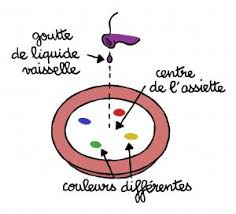
\includegraphics[width=0.35\textwidth]{images/LaitColorants.jpg}
    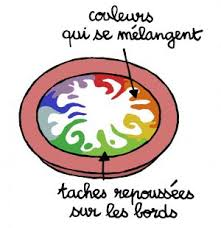
\includegraphics[width=0.26\textwidth]{images/LaitColorants2.jpg}
\end{figure}


\end{exo}


\begin{exo}["Le passé est un œuf cassé, l'avenir est un œuf couvé."]
Pour éviter de casser des œufs, évitons de les toucher ! Il faut néanmoins écailler l’œuf dur... comment faire ?

Pire encore, pour conserver les œufs, rien de mieux que de les mettre en bouteille (de verre, bien sûr, c'est plus solide et plus stérile). Par contre, vous vous êtes trompé de bouteille : son goulot est trop petit. En appuyant très fort, l’œuf peut rentrer, oui, mais sans les toucher, ça relève du défi. Heureusement, vous êtes là pour relever ce défi !


\begin{figure}[h!]
	\centering
    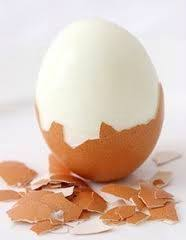
\includegraphics[width=0.2\textwidth]{images/OeufEcaille.jpg}
    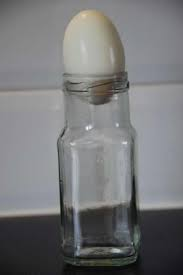
\includegraphics[width=0.17\textwidth]{images/OeufEnBouteille.jpg}
\end{figure}
\end{exo}


\begin{exo}[En coupant un cube]
On coupe un cube par un plan. Quelles sont les sections possibles ? Comment obtenir une section de périmètre maximal ? D'aire maximale ?

\begin{figure}[h!]
	\centering
    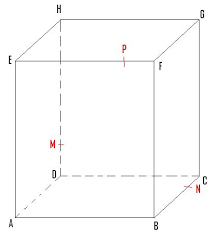
\includegraphics[width=0.17\textwidth]{images/Cube.png}
    
\end{figure}
\end{exo}


\begin{exo}[Dans le coin de l'ennui]
Edwige s'ennuie en cours de mathématiques. Elle sort alors sa règle et commence à jouer avec : elle la place au coin de sa table et la fait bouger, créant ainsi diverses figures. Elle se pose la question suivante : << Si je prend ma règle et que je joins les deux bords de mon coin de table, quelle est l'aire du plus grand triangle que je puisse former ? >>

\begin{figure}[h!]
	\centering
    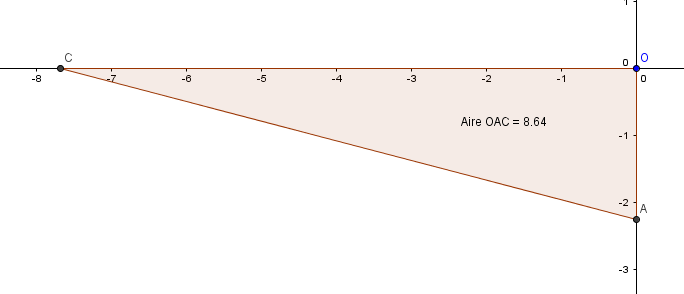
\includegraphics[width=0.7\textwidth]{images/TriangleCoinDeTable.png}
    
\end{figure}
\end{exo}


\begin{exo}[Sous la courbe, un rectangle]
Soit $C_f$ le graphe d'une fonction f homographique. On repère le centre du graphe, puis on trace un rectangle entre ce dernier et un point quelconque de $C_f$. On mesure l'aire de ce rectangle. On change de point sur la courbe, on construit à nouveau le rectangle, on en mesure à nouveau l'aire : on trouve la même valeur!

Expliquez ce phénomène.

\begin{figure}[h!]
	\centering
    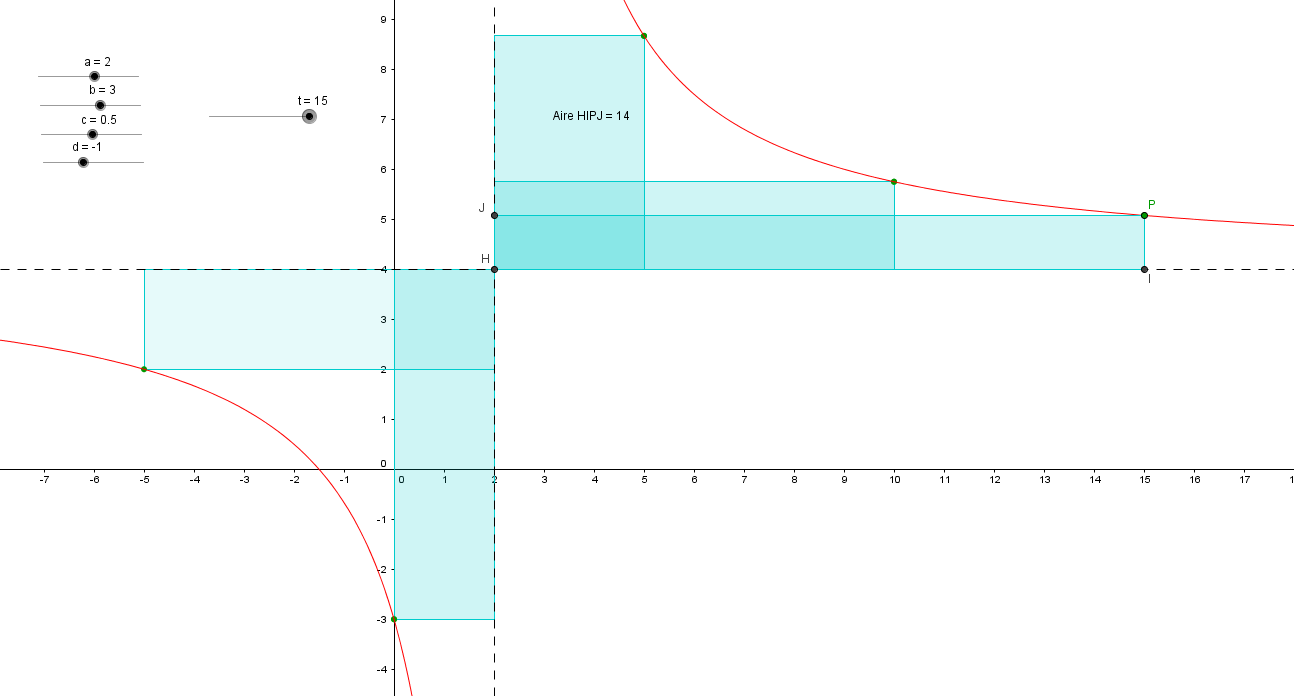
\includegraphics[width=0.7\textwidth]{images/RectangleHomographique.png}
    
\end{figure}
\end{exo}


\begin{exo}[Triple cercle]
On trace trois cercles tangents de centres alignés et de même rayon. On trace le segment passant par les trois centres. On choisit un angle $\theta$, et on place sur chaque cercle le point à $\theta$ radians. Pour chacun de ces trois points, on trace le segment le reliant au(x) centre(s) du (des) cercle(s) voisin(s).

On obtient une figure centrale qui semble être un quadrilatère particulier. Le reconnaissez-vous ? Démontrez que, quelque soit $\theta$, ce quadrilatère est bien particulier, puis calculez son aire en fonction du rayon $R$ des cercles et de l'angle $\theta$.

\begin{figure}[h!]
	\centering
    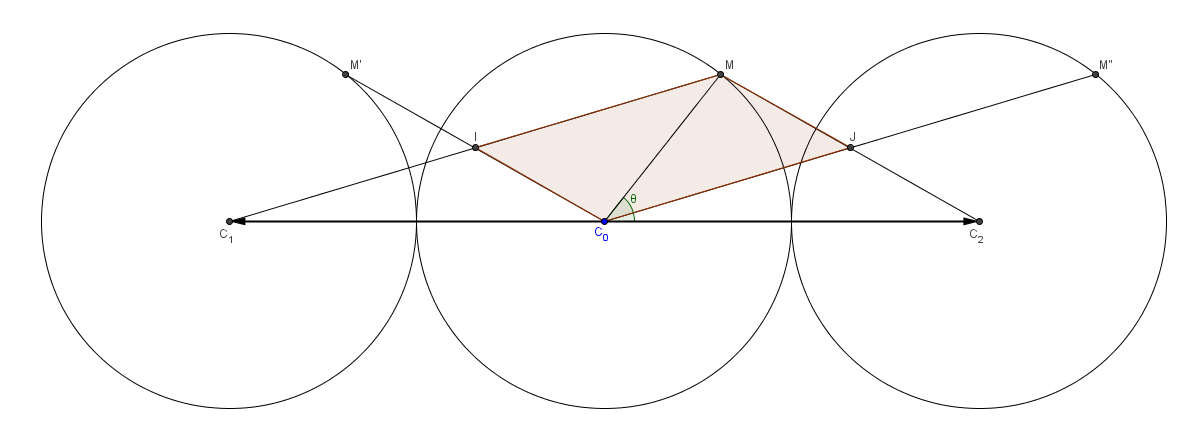
\includegraphics[width=0.7\textwidth]{images/TripleCercle.png}
    
\end{figure}
\end{exo}


\begin{exo}[Un carré dans la parabole]
On prend une parabole, branches vers le haut. On nomme A son sommet, et on place un point mobile B sur la branche de droite. On trace le segment [AB], puis on construit le carré engendré par ce segment. Pour deux positions bien spécifiques du point B, le carré construit a 3 sommets sur la parabole. Calculez les aires correspondant à ces deux situations.


\begin{figure}[h!]
	\centering
    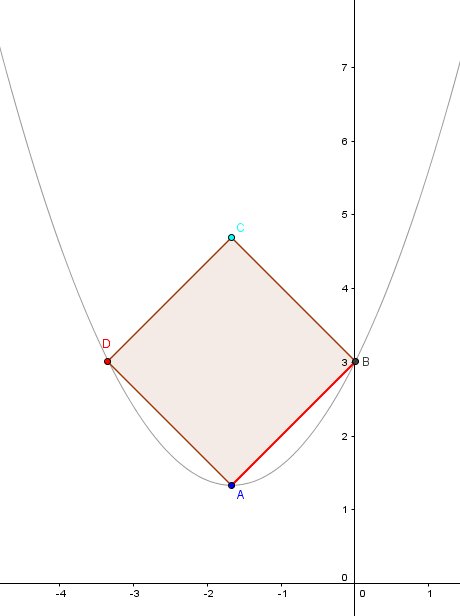
\includegraphics[width=0.35\textwidth]{images/CarreParabole.png}
    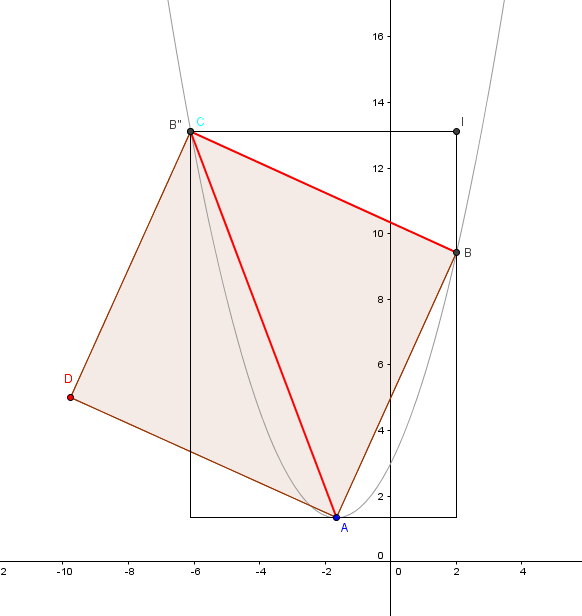
\includegraphics[width=0.4\textwidth]{images/CarreParabole2.png}
\end{figure}
\end{exo}


\begin{exo}[Le sommet de la parabole]
On trace une parabole quelconque d'équation $aX^2+bX+c$. On marque le sommet, puis, à $b$ et $c$ fixés, on fait varier $a$ de $-\infty$ à $+\infty$. On regarde la figure obtenue. On recommence en fixant $a$ et $c$ et on fait varier $b$. Enfin, on trace la courbe obtenue en faisant varier $c$.

Sur le dessin qui suit, identifiez quelle courbe correspond à quelle variable. Déterminez les équations qui correspondent à chaque courbe (en fonction de $a$, $b$ et $c$). Il est conseillé de commencer par la courbe engendrée par les variations de $c$, puis celles de $a$, et enfin de $b$.

\begin{figure}[h!]
	\centering
    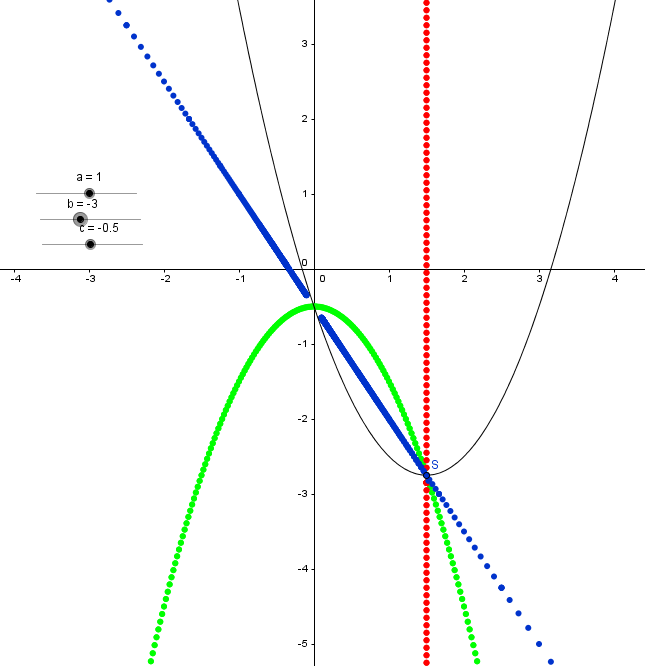
\includegraphics[width=0.5\textwidth]{images/SommetParabole.png}

\end{figure}
\end{exo}


\begin{exo}[Le paradoxe des Monty Hall]
Un présentateur TV facétieux vous a organisé un petit jeu. Vous êtes placé devant trois portes fermées. Derrière l'une d'elles se trouve une voiture et derrière chacune des deux autres se trouve une chèvre. Tout d'abord, on vous demande de désigner une porte, puis le présentateur ouvre une porte qui n'est pas celle que vous avez choisie, et qui cache une chèvre. Vous avez a alors le droit ou bien d'ouvrir la porte choisie initialement, ou bien de changer de porte pour ouvrir la troisième.

Que devez-vous faire ? Quelles sont vos chances de gagner la voiture ?

\begin{figure}[!ht]
	\centering
    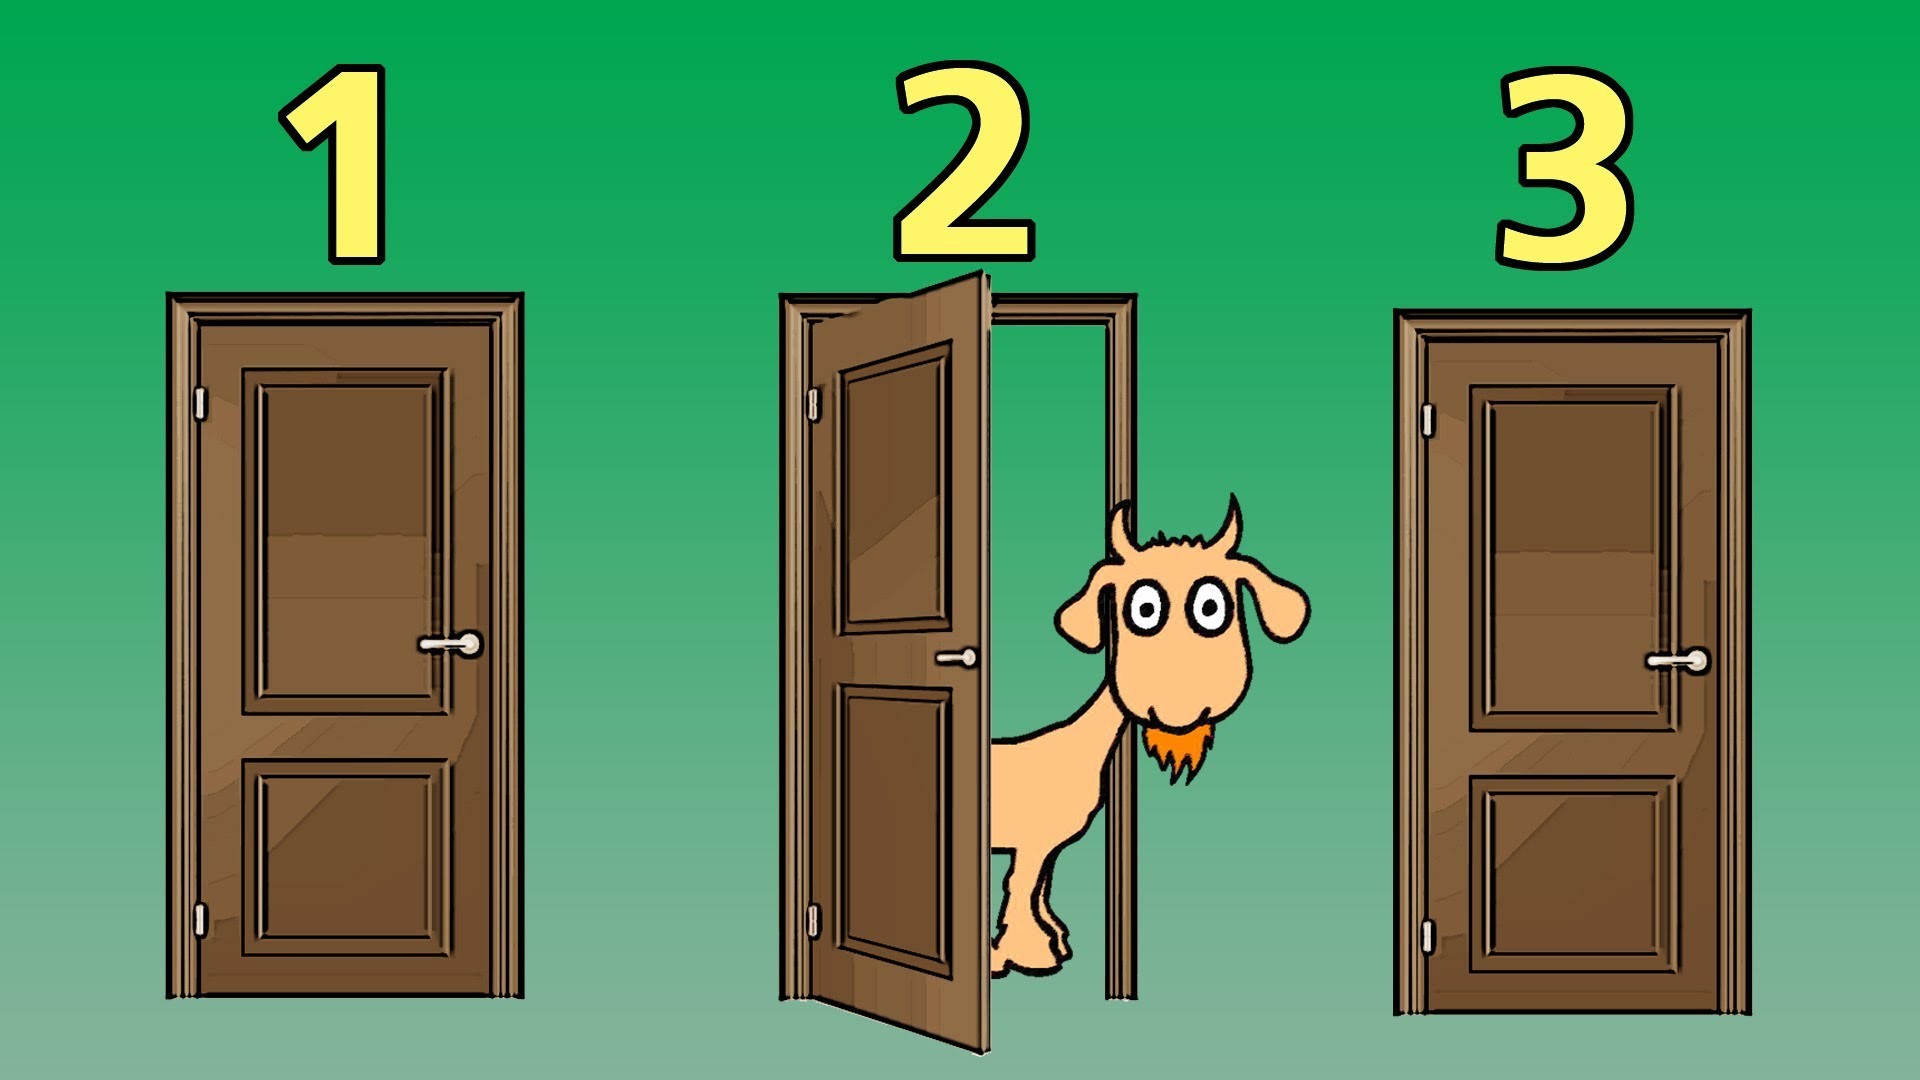
\includegraphics[width=0.55\textwidth]{images/MontyHall.jpg}

\end{figure}
\end{exo}


\begin{exo}[L'escargot face au Géant]
Un escargot avance lentement, disons à $v = 5 cm.h^{-1}$ sur un élastique magique. Il part de la gauche, alors qu'à droite, un Géant, aussi oisif que patient, allonge toutes les heures l'élastique d'une longueur $l = 1 m$.

L'escargot atteindra-t-il un jour le bout de l'élastique ? Si oui, en combien de temps ?
\begin{figure}[!ht]
	\centering
    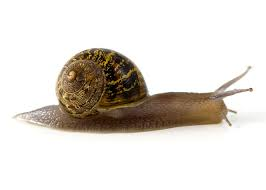
\includegraphics[width=0.2\textwidth]{images/Escargot.jpg}
    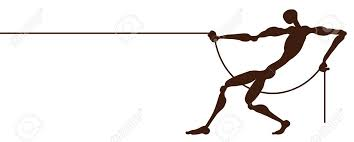
\includegraphics[width=0.4\textwidth]{images/Geant.jpg}

\end{figure}
\end{exo}


\begin{exo}[Solides de Platon]
Vous connaissez des solides réguliers ? Combien en connaissez-vous ? Comment démontrer qu'il n'y en a pas d'autres ?

\begin{figure}[!ht]
	\centering
    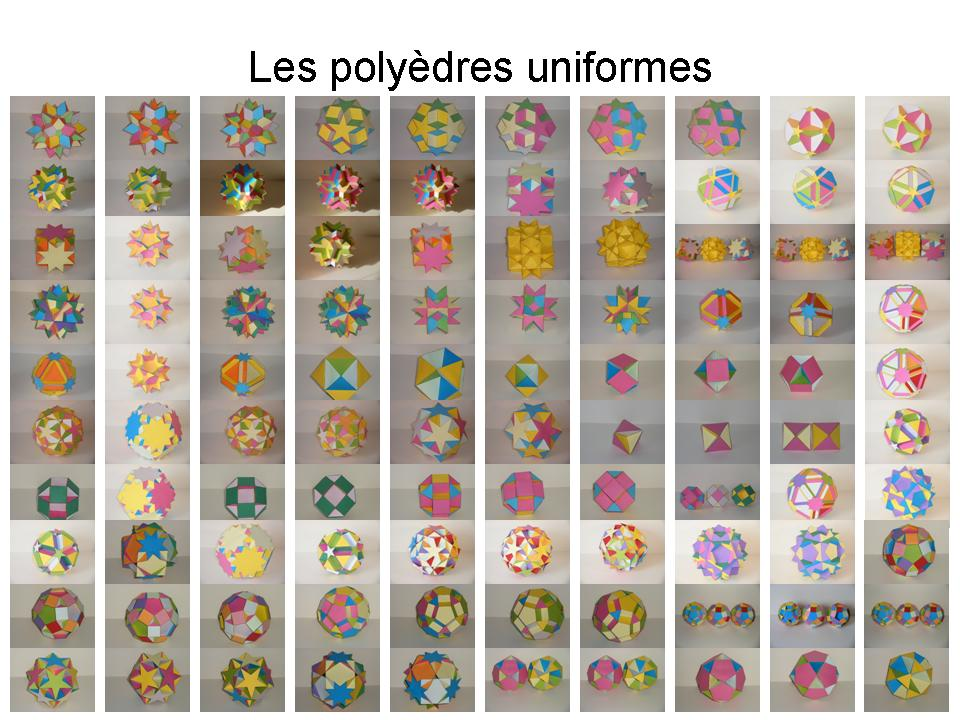
\includegraphics[width=0.95\textwidth]{images/PolyedreUniforme.jpg}

\end{figure}
\end{exo}


\pagebreak

%%%%%%%%%%% CORRECTIONS %%%%%%%%%%%%%

\section*{Corrections des exercices}

\begin{cor}
\textit{L'exercice peut se traiter comme un exercice d'arithmétique modulaire avec une équation diophantienne, ou encore comme un exercice de géométrie dans le plan, en effectuant le tracé de la droite d'équation cartésienne $3x + 5y = 40$ et en identifiant les points à coordonnées entières.}\newline



\textit{Mise en équation; Pratique du second degré; Exercice classique; Non unicité des solutions...}
\end{cor}


\begin{cor}
La stratégie \textit{naïve} consiste en sélectionner le plus petit élément de la liste, le permuter avec l'élément en dernière position, et recommencer sur les $n-1$ derniers éléments de la liste résultat.

Bien sûr, il faut d'abord définir un algorithme permettant de sélectionner le plus petit élément d'une liste: cela se fait avec un ordre de grandeur de $n$ opérations.\newline



Voici une implémentation d'un tel algorithme dans le langage \verb|Python|:

\begin{lstlisting}
def min_liste(l):
	n = l.length
	indMin = 0
    for i in range(1,n):
    	if l[indMin] < l[i]:
        	indMin = i
    return indMin

def tri_liste(l):
	n = l.length
    for i in range(n):
    	indMin = min_liste(l[i:])
        l[i], l[indMin] = l[indMin], l[i]
\end{lstlisting} 


Finalement, on obtient un algorithme de tri, appelé \textit{tri par sélection (du minimum)} qui fait de l'ordre de $n^2$ opérations. C'est un bon début pour un débutant en algorithmique, mais on peut faire bien mieux\ldots

Vidéo illustrant le tri par minimum : \url{https://www.youtube.com/watch?v=0-W8OEwLebQ}
\newline

\textit{Initiation à la programmation; Premiers raisonnements par algorithmes; Formalisme; Rigueur...}
\end{cor}


\begin{cor}[Tasse de café et tasse de lait]
\textit{Ramener des verres en plastique pour faire l'expérience.}

\textit{La taille de la cuillère est-elle importante ? Que se passe-il quand on change sa taille ?}

3 stratégies de réponses peuvent être présentées. Toutes démontrent qu'il y a autant de lait dans la tasse de café que de café dans la tasse de lait.
\newline \newline


\underline{Première méthode : symétrie}

Mettons qu'on obtienne qu'il y a plus de café dans le lait que de lait dans le café. Recommençons l'expérience en inversant seulement la position initiale des tasses : on obtient alors l'inégalité contraire. Du coup, il y a égalité.\newline



\textit{Symétrie d'une relation d'ordre; Raisonnement par double implication...}
\newline

\underline{Deuxième méthode : invariant de cuillère}

Est-ce que la taille de la cuillère influence le résultat ? Non ! Donc je peux soit prendre une cuillère de volume nul, soit une de volume égal à celui d'une tasse. Dès lors, il y a autant de lait dans le café que de café dans le lait.

\textit{Continuité, constance; Raisonnements sur des invariants}
\newline

\underline{Troisième méthode : calcul de la concentration}

On peut calculer les 6 nombres importants à chaque étape du processus : concentration en café, concentration en lait et volume de liquide dans chaque tasse. Après des calculs casse-pieds, on s'en sort avec les mêmes concentrations des deux côtés.

\textit{Identifications des paramètres clés; Mise en place de méthodes de calcul; Concentrations, quantité et volumes; Rigueur de calcul}
\end{cor}


\begin{cor}
\textit{Ramener un plateau d'échecs avec 3 cavaliers de chaque couleur si possible. Ramener un ordinateur avec ChessBase.}

\textit{Indication :
Une option possible est de noter combien de déplacements sont nécessaires pour passer d'une case x à une case y, et ce pour toutes les cases de l'échiquier.}

Vidéo d'explication du problème (avec les solutions des nombres de coup) : \url{https://www.youtube.com/watch?v=YfI7iQrqKGg}\newline


Vidéo qui décortique la modélisation de l'échiquier pour le cavalier : \url{https://www.youtube.com/watch?v=HcUvd-v6x0o}\newline

\textit{Changement de perspective ; Voir le monde selon le point de vue du cavalier ; Nouvelle modélisation = nouvelles informations ; Introduction aux jeux mathématisés; Faire une partie d'échecs ?}
\end{cor}


\begin{cor}
\textit{Cet exercice, en plus de susciter des exclamations de joie surprise, introduit la théorie de l'information, de l'encodage et de la compression de données.}\newline

\textit{Les deux magiciens ont vraisemblablement un code pour communiquer à travers les 4 cartes visibles... Comment feriez-vous à leur place ?}\newline

Pour réaliser ce tour, il faut noter qu'à chaque étape, c'est le magicien dans la pièce qui organise les choses. C'est lui qui choisi quelle carte est dissimulée et comment sont disposées les 4 autres cartes. Cela va permettre de transmettre un message au magicien resté à l'extérieur.

Tout d'abord, 5 cartes sont piochées. D'après le principe de \textsc{Dirichlet} (principe des tiroirs), 2 au moins sont de la même couleur. Le magicien en confie une pour qu'elle soit dissimulée et met l'autre sur la table, le plus près de la porte. Celui qui entre saura immédiatement de quelle couleur est la carte qu'il doit identifier (pique, trèfle, cœur ou carreau). Ensuite, il reste à identifier laquelle des 12 cartes (l'une étant déjà sortie sur la table) est la bonne.

Celui resté dans la salle dispose de 3 cartes pour coder 12 informations de manière unique. Il peut par exemple se servir des permutations de $S_{3}$. En définissant un ordre sur les cartes, on les numérote dans sa tête 1, 2 et 3, puis on les mélange pour coder pour les nombres de 1 à 6 ($\#S_{3} = 6$). En jouant sur l'orientation de la première carte (horizontale ou verticale par exemple), on double le nombre d'information possible. Il n'y a plus qu'à se mettre d'accord ensemble à l'avance et à bien réviser !\newline

\textit{Introduction à la cryptologie ; Introduction aux permutations ; Introduction aux clé publique / clé privée ; Introduction à l'oral de l'Ulm ; Introduction à l'art d'illusionner le public}
\end{cor}


\begin{cor}
\textit{Comment feriez-vous pour retrouver le jour de la semaine du 1er du mois dernier ?}

Un peu de culture pour commencer : la prise de la Bastille a eu lieu le... 14 juillet 1789 ! Le tableau de gauche est un \textsc{Eugène Delacroix} et celui de droite un \textsc{Jean-Pierre Houël}.\newline

Pour trouver le jour de la semaine correspondant, on commence par trouver que jour de la semaine tombe le 14 juillet de l'année en cours, puis on utilise le fait que $365 = 1 [7]$ pour dire que chaque année en arrière fait remonter d'un jour dans la semaine. Reste à prendre en compte les années bissextiles (sachant qu'elles sont multiple de 4 mais pas de 400 sauf de 2000). \textbf{Il est conseillé de commencer par calculer le jour de la semaine de sa naissance.} La prise de la Bastille a eu lieu un mardi.\newline \newline

\textit{Introduction à l'arithmétique modulaire, au programme de Spé Maths ; Mener des calculs qui se complexifient ; Chercher par soi-même ; Connaissance des années bissextiles ; Culture générale}
\end{cor}


\begin{cor}
On pourra utiliser la page suivante : \url{https://fr.wikipedia.org/wiki/Paradoxe_des_anniversaires}\newline

On peut commencer par calculer la probabilité que 2 personnes aient leurs anniversaires le même jour : la méthode la plus simple est alors de calculer la probabilité qu'ils n'aient pas leur anniversaire le même jour. On a 365 possibilités pour l'anniversaire du premier (on néglige les années bissextiles), il reste donc 364 jours pour la seconde personne. La probabilité qu'ils aient leur anniversaire le même jours est donc \[
\PP(Anniveraire_1 \neq Anniversaire_2) = 1 - \frac{1}{365} = \frac{364}{365}. 
\]
Pour $n$ personnes maintenant, si on veut calculer le nombres de possibilités pour que ces $n$ personnes aient $n$ jours d'anniversaire différents, on obtient des arrangement de $n$ parmi $365$ :\[
 (365 - 0)(365 - 1)...(365 - n + 1) = \frac{(365)!}{(365 - n)!} 
\]

Maintenant qu'on connaît le nombre de cas satisfaisant notre exigence, on divise par le nombre total de cas possibles pour obtenir la probabilité d'avoir $n$ anniversaires qui tombent $n$ jours différents :
\[
 1 - \PP(n) =  \frac{(365)!}{(365 - n)!} . \frac{1}{365^n}
\]
On peut aussi voir cela comme une multiplication de probabilités d'événements : les probabilités que l'anniversaire de la $i$-ème personne ne tombe pas sur un des jours déjà occupé par l'anniversaire d'une des $(i-1)$-èmes personnes précédentes :
\[
 1 - \PP(n) =  \frac{365}{365}  . \frac{365 - 1 }{365} ...  \frac{365-n + 1 }{365}
\]

Soit 
\[
 \PP(n) = 1 - \frac{365}{365}  * \frac{365 - 1 }{365} * ... * \frac{365-n + 1 }{365}
\]

Quand $n$ devient grand, on peut trouver une fonction équivalente à cette probabilité (passer au logarithme, on obtient une somme, utiliser l'équivalent $ln(1+x) \~ x$, sommer et on obtient la formule qui suit) : \[
\PP(n) \approx 1 - \exp{(- \frac{n(n-1)}{2 * 365})}
\]
On peut donc en déduire le nombre de personne que l'on doit réunir pour avoir une probabilité donnée $p$ de trouver deux personnes ayant leurs anniversaires le même jour (en calculant la fonction réciproque) :
\[ 
n(p) \approx \sqrt[]{2 * 365 \log{ \frac{1}{1-p}} }
\]

Le nombre de personnes à réunir pour que l'on ait une chance sur deux d'obtenir deux anniversaires le même jour est donc 23 personnes environ. \newline

\textit{Dénombrement ; Principe des tiroirs ; Réflexion par la contraposée ; Approximation du résultat ; Fonctions exponentielles et logarithme (Terminale)}
\end{cor}


\begin{cor}
\textit{Que se passe-t-il si vous coupez le long d'une arrête ?}

L'idée est de mettre en place une démarche progressive. D'abord on se demande si le plan de coupe peut passer par un seul sommet (non, sans quoi une partie contiendrait deux sommets et l'autre un seul). Peut-il passer par 2 sommets (non, les deux parties sont alors chirales). Dès lors, le plan ne passe par aucun sommet. Pour des raisons de symétrie, il doit en plus passer par toutes les arrêtes et toutes les faces.

On teste enfin la coupe restante la plus logique : celle qui passe par les milieux de chaque arrête, et ça marche ! On peut noter au passage que la section coupé est un carré : ce n'est pas un hasard de trouver un polygone régulier.

\begin{figure}[h!]
	\centering
    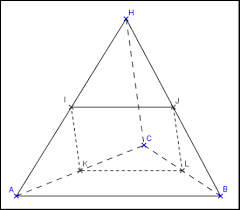
\includegraphics[width=0.3\textwidth]{images/CoupeTetraedreAvecSolution.png}
    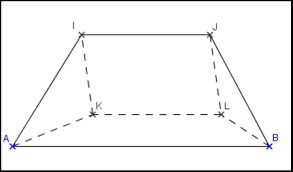
\includegraphics[width=0.45\textwidth]{images/CoupeTetraedreAvecSolution2.png}
\end{figure}

\textit{Visualisation dans l'espace; Introduction à la géométrie dans l'espace; Mise en place de raisonnements logiques pour simplifer un problème.}

\end{cor}


\begin{cor}
\textit{Il s'agit évidemment d'un exercice de probabilités sur les variables aléatoires. L'effort de formalisation porte surtout sur modéliser correctement le déplacement de l'ivrogne par une suite de variables de Rademacher.}

On note $X_t$ la position de Jean-Michel à l'instant $t\in\NN$: c'est une variable aléatoire réelle discrète puisqu'il se déplace d'une unité à chaque instant.

Le déplacement entre les instants $t-1$ et $t$ est la variable aléatoire $\xi_t := X_t-X_{t-1}$. Cette variable aléatoire suit la loi de probabilité
\[
\PP(\xi_t = 1) = \PP(\xi_t = -1) = \frac{1}{2}. 
\]
Cette variable aléatoire finie admet pour espérance $\EE(\xi_t) = 0$, et les variables $(\xi_t)_{t\geq 0}$ suivent la même loi et sont indépendantes.

Un calcul simple montre que la position de Jean-Michel à l'instant $t$ est:
\[
X_t = \sum_{k=1}^t \xi_k,
\]
donc que son espérance mathématique, la position moyenne de Jean-Michel, est $\EE(X_t) = 0$.

\textit{La deuxième question, plus ambiguë, fait appel à quelques notions de statistiques, et peut servir d'introduction au théorème central limite pour faire le pont entre les probabilités et la maigre introduction aux statistiques en classe de Seconde.}

On cherche à donner un encadrement des positions successives $X_t$ de Jean-Michel qui soit vérifié dans la majeure partie des cas.

La variance de $X_t$ est donnée par la somme des variances des $(\xi_t)_{t\geq 0}$, qui valent $1$:
\[
\VV(X_t) = \sum_{k=1}^t \VV(\xi_k) = t.
\]
L'écart-type est donc $\sigma(X_t) = \sqrt{t}$.

On a d'après le théorème central limite
\[
\frac{X_t}{\sqrt{t}} \xrightarrow[t\to\infty]{\PP} N
\]
où $N$ est une variable normale centrée réduite.

\textit{Il faut donc introduire la notion de convergence en loi d'une variable aléatoire.}

L'intuition suggère qu'après $t$ pas, la position de Jean-Michel serait bornée par l'écart-type $\sigma(X_t)$. Cherchons donc une constante positive $c > 0$ telle que $|X_t| \leq c\sqrt{t}$ avec une << bonne certitude >> :
\[
\PP\left(-c\sqrt t \leq X_t \leq c\sqrt t\right) = 0,\!99
\]
ce qui donne sur le temps long $\PP(-c \leq N \leq c) = 0,\!99$ soit $2\Phi(c) - 1 = 0,\!99$ où $\Phi$ est la fonction de répartition de la loi normale centrée réduite. On obtient alors $c\approx 1,\!98$.\newline 

\textit{Pratique des probabilités; Effort de formalisation; Notion de convergence; Résultats classiques : Jean-Michel va passer une infinité de fois par tous les points du plan.}

\end{cor}


\begin{cor}
Cet exercice est assez difficile et demande à ce que les calculs soient menés avec dextérité, intelligence et concentration.

La première étape est de mettre en équation (en fonction en l'occurrence) la position au cours du temps de la grande aiguille, puis de la petite. Prenons 00h00 pour position initiale.

La grande aiguille avance à une vitesse de 1 tour par 12 heures. Il y a 5 minutes d'arc par heure, soit 60 minutes d'arc en tout, donc la grande aiguille avance de 60' en 12 heure, soit en 12*60 minutes. Il lui faut donc 12 minutes pour avancer de 1' : elle avance à la vitesse angulaire $\Omega = 1/12 '.min^{-1}$.

La petite aiguille, quand à elle parcourt par définition 1' par minute : $\omega = 1 '.min^{-1}$.

La position au cour du temps de la grande aiguille est donc donnée en minute d'arc par : $\Theta(t) = \Omega t + \Theta(t=0) = \Omega t = t/12$, où $t$ est en minute. Celle de la petite aiguille est donnée par : $\theta(t) = \omega t + \theta(t=0) = \omega t = t$.

On veut que les aiguilles soient perpendiculaires, c'est-à-dire : $\theta(t) - \Theta(t) = \pm 15' [60]$. On obtient l'équation à deux variables ($t \in \textbf{R}$ et $h \in [|0, 11|]$) : $(1-1/12) t = \pm 15 + 60h$. Ainsi : $t = (180/11) * (4 h \pm 1)$.

On obtient ainsi les 22 positions possibles :\begin{itemize}
\item 11h43,63 et 00h16,36 
\item 00h49,09 et 1h21,81
\item 1h54,54 et 2h27,27
\item \textbf{3h00} et 3h32,72
\item 4h05,45 et 4h38,18
\item 5h10,90 et 5h43,63
\item 6h16,36 et 6h49,09
\item 7h21,81 et 7h54,54
\item 8h27,27 et \textbf{9h00}
\item 9h32,72 et 10h05,45
\item 10h38,18 et 11h10,09
\end{itemize}

Pour un angle quelconque entre les aiguilles, il suffit de remplacer dans les équations le "$\pm 15$" par l'angle voulu en minute d'arc.\newline 

\textit{Travail de concentration ; Angles orientés ; Arithmétique modulaire ; Dessin, visualisation et imagination}
\end{cor}


\begin{cor}
\textit{Où voulez-vous placer la plus grande crêpe ? Et la plus petite ? Comment vous y prendre ?}

Le plus simple est de présenter un algorithme récursif. L'idée principale est d'amener la plus grande crêpe en bas de la pile : on repère la plus grande crêpe dans la pile, on place la spatule juste en dessous, puis on retourne le haut. La plus grande crêpe est alors tout en haut de la pile. Il suffit de retourner la totalité de la pile (en mettant la spatule tout en dessous), pour que la plus grande crêpe soit en bas. 

On recommence avec les $71$ crêpes supérieurs pour mettre la deuxième plus grande sur la première plus grande, puis avec les $70$ supérieurs, etc. En fait, on trie la pile récursivement.

Pour calculer la complexité, on remarque qu'il faut 2 étapes pour mettre une grande crêpe en bas, donc il faut $2n$ retournements (au pire) pour trier la pile.

\textit{Introduction à la récursivité ; Dessin, visualisation et imagination ; Introduction à la complexité ; Introduction aux maths dans le quotidien}
\end{cor}


\begin{cor}
\textit{Vous pouvez d'abord raisonner avec un nombre réduit de disques.}

C'est exercice est assez classique, il poursuit le précédent. Là encore, il s'agit de récursivité.

Commençons par apprendre à déplacer la plus grosse pierre du bâton de gauche à celui de droite. Raisonnons par récurrence. Si on sait déplacer une tour de n disques. Pour déplacer une tour de n+1 disques, on déplace les n disques supérieurs sur le bâton central, puis on déplace le plus grand disque maintenant libre sur le bâton de gauche, et on déplace à nouveau les n disques du bâton central sur celui de gauche. L'ensemble de la tour à bien été déplacée.

La complexité se calcul par récurrence : $C_{n+1} = C_n + 1 + C_n$. En posant $u_n = C_n + 1$, on a $u_{n+1} = 2u_n$, puis $u_n = 2^n$ (car $u_1 = C_1 + 1 = 1+1 + 2$) et enfin $C_n = 2^n + 1$.\newline 

\textit{Introduction à la récursivité ; Dessin, visualisation et imagination ; Introduction à la complexité ; Introduction aux maths dans le quotidien ; Culture mathématique}
\end{cor}


\begin{cor}
On pourra commencer par rappeler qui est le père Fouettard. Pour rendre cet exercice ludique, on ferme les deux battants du tableau, puis on dessine une porte sur chacun. derrière ces battants, on dessine d'un côté le père Noël et de l'autre le père Fouettard. Les deux membres du binôme se placent chacun devant un battant du tableau.

En posant la question, il faut réussir à obtenir une information indépendante de la situation. Il y a quatre situations possibles :\begin{enumerate}
\item Germain est devant chez le père Noël et ment.
\item Suzie est devant chez le père Noël et ment.
\item Germain est devant chez le père Noël et dit la vérité.
\item Suzie est devant chez le père Noël et dit la vérité.
\end{enumerate}

Pour obtenir une phrase qui ne dépend plus de la situation, il faut créer un invariant : impliquer et Germain et Suzie dans une même phrase. Par exemple, on va voir Suzie et on lui demande : << Est-ce que Germain m'aurait dit que je suis devant chez le père Noël ? >>. En impliquant ainsi les deux gardiens, on "somme" le mensonge et la bonne foi, permettant d'obtenir une information, non pas fiable, mais prévisible, dont on peut extraire l'information voulue. Le même principe se retrouve lorsqu'on s'intéresse au point fixe d'une application ou à la somme d'un ensemble : on somme des informations pour faire disparaître leur particularités dont on ignore tout dans la masse sur laquelle on peut alors travailler.

\textit{Théorie des invariants ; Casse-tête logique ; Jeux en classe}
\end{cor}


\begin{cor}
\textit{Si on fait la somme des gains de chacun, quelle stratégie est la meilleure pour l'ensemble du groupe ? Et en ne considérant que vos gains personnels ? Prenez aussi en compte le fait que l'autre joueur cherche lui aussi à maximiser son gain personnel.}

Il n'y a pas vraiment de correction. La meilleur stratégie, nommée "Copycat" consiste à copier l'adversaire : on commence par coopérer et ensuite on joue le dernier coup de l'opposant (s'il vient de nous trahir, on trahi, sinon on coopère). Pour les différentes stratégies intéressantes, voir cette vidéo : \url{https://www.youtube.com/watch?v=StRqGx9ri2I}

L'un des deux membres du binôme peut jouer la stratégie méchante et l'autre le Copycat. Les élèves devront alors faire la différence entre gagner le plus de matches et gagner au total (le plus d'argent). \newline

\textit{Introduction à la théorie de jeux ; Initiative personnelle ; Sensibilisation sur le quotidien, aux débats de société ; Jeu à somme non constante ; Différence entre gagner ponctuellement et gagner au total}
\end{cor}


\begin{cor}
\textit{Concrètement, qu'implique la différence de densité quand on considère un même volume d'eau chaude et d'eau froide ? Et quand on raisonne par rapport à une même masse ? Quelles sont les conséquences au niveau moléculaire ?}

Il y a plusieurs méthodes possibles, le but est que les élèves proposent des méthodes peu banales. Deux méthodes sont "classiques" : les colorants (on colore l'eau froide en bleu et l'eau chaude en rouge, en versant dans un aquarium d'eau tempérée, on voit la séparation) et la salinité (comme elle est dilatée, l'eau chaude peut accueillir plus de sel que l'eau froide, il suffit de mesurer la saturation des deux).

\textit{Initiative personnelle ; Protocole expérimental ; Dilatation et contraction ; Représentation concrète d'un phénomène étudié en classe; Think outside the boxe}
\end{cor}


\begin{cor}
\textit{Vous vous souvenez de la formule du périmètre d'un disque ?}

On pourrait croire que qu'il suffit d'un seul tour, mais il en faut deux : on peut par exemple regarder le mouvement du centre de la pièce extérieure. Il parcourt un cercle de rayon 2, donc doit faire 2 tours.

Bonne chance pour expliquer cela correctement aux élèves !\newline 

\textit{Imagination ; Combattre ses préjugés ; Jeu; utilisation des formules vues en cours.}
\end{cor}


\begin{cor}
De la même manière que pour l'exercice précédent, le plus simple est de regarder l'augmentation de rayon : comme elle est identique dans les deux cas, la circonférence augmente de $2\pi$, donc l'augmentation est identique.

Par contre, l'aire et le volume ne sont pas linéaires en R (le rayon), donc l'augmentation ne sera pas identique.\newline 

\textit{Introduction aux processus linéaires ; Importance ou non de la taille de départ ; Illusion de simplicité}
\end{cor}


\begin{cor}

Le lait contient de l’eau, mais aussi du gras sous forme de petites gouttes. Comme le gras et le colorant ne se mélangent pas, les taches restent bien rondes ! Quand on met le liquide vaisselle, il perturbe les molécules de gras à la surface du lait, au centre de l’assiette… Cela repousse le colorant vers les bords. En plus, le savon se fixe sur le gras et augmente sa miscibilité avec l'eau (C'est pour ça que l'on se lave les mains avec du savon !). Le colorant peut alors se mélanger plus facilement avec le lait !

\textit{Introduction à la génétique; Culture générale; Introduction à la chimie et à la biologie cellulaire; YouTube comme outil pédagogique; Experience étonnante et amusante. }

\end{cor}


\begin{cor}
\textit{La citation qui sert de titre à l'exercice est de \textsc{Paul Éluard}.} \newline

\textit{Vaut-il mieux pousser l’œuf ou le faire rentrer en l'aspirant à l'intérieur de la bouteille ? Une fois que vous aurez tranché, comment pourriez-vous vous y prendre concrètement ? N'hésitez pas à proposer tout le matériel que vous imaginez !}

Pour dissoudre la coquille de l’œuf, on utilise du vinaigre. Le vinaigre, très acide, permet de "cuire" les aliments. La coquille est dissoute, et ensuite l'albumine (le blanc) est dénaturé, et se solidifie en surface en une seconde coquille. On obtient un œuf presque cru (il a été un peu chauffé par la réaction néanmoins), entouré par une membrane souple : c'est une balle rebondissante !

Ensuite, pour faire rentrer un œuf dur dans une bouteille de verre, il suffit de chauffer l'air intérieur qui, en refroidissant se contracte et aspire l’œuf.\newline 

\begin{figure}[!ht]
	\centering
    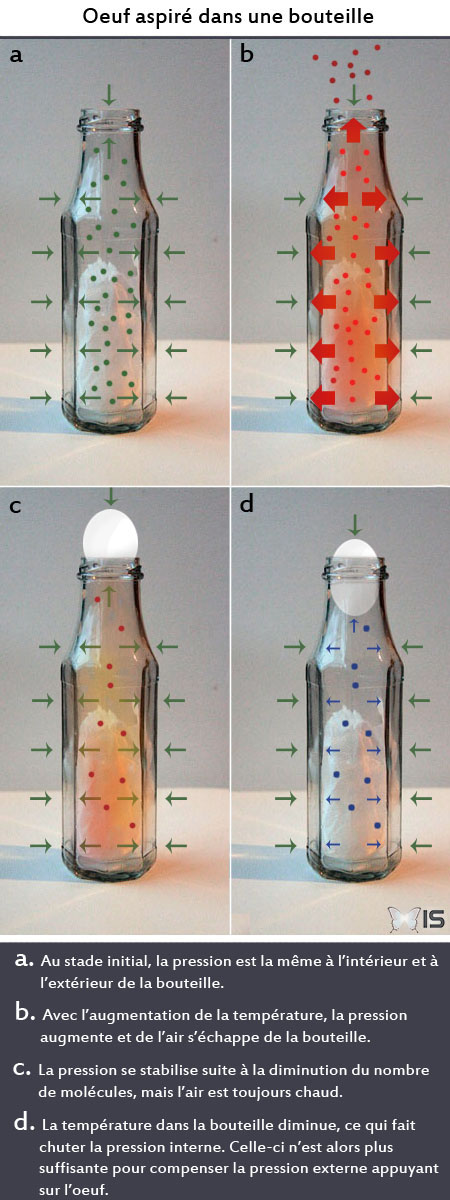
\includegraphics[width=0.35\textwidth]{images/ExplicationOeuf.jpg}
    
\end{figure}

 \textit{Protocole scientifique ; Mécanique des fluides ; Dilatation et contraction ; Chimie acido-basique ; Méthode de cuisson ; Macération ;Cuisine moléculaire ; Jeux}
\end{cor}


\begin{cor}
Il existe plein de manières de couper un cube. On peut faire des triangles (quelconques, isocèles, équilatéraux ou rectangle), des quadrilatères (quelconques, rectangles ou carrés), des pentagones (réguliers ou non), et des hexagones (réguliers ou non). En faisant un hexagone qui passe par le milieu de chaque face, on obtient un figure de périmètre $3c \sqrt{2}$, ce qui est le maximum (je n'ai pas vérifié). L'aire obtenue est de $3c \sqrt{3}/4$.

\textit{Raisonnement en 3 dimensions; Utilisation de la logique sur des problèmes complexes; Rigueur des raisonnments.}

\end{cor}


\begin{cor}
En utilisant le théorème de Pythagore, on obtient la longueur du second côté du coin : $\sqrt{l^2 - x^2}$. Ensuite, l'aire obtenue vaut $A(x) = x \sqrt{l^2 - x^2}$. Dès lors, le plus simple pour obtenir le maximum de $A(x)$ est de calculer $f = A^2$ en fonction $t = x^2$.

On obtient :

$f(t) = t(l^2-t)$, donc on a une forme factorisée d'un polynôme du second degré, son extremum (qui est bien un maximum) est atteint en $t = l^2/2$, c'est-à-dire $x = l \sqrt{2}/2$, donc $A = l^2/4$.

On obtient bien ainsi l'unique maximum de $A$ car l'application $x \rightarrow \sqrt{x}$ est croissante dont son application ne change pas les variations.

On aurait pu se servir d'arguments de symétrie, qui démontre qu'il y au moins un maximum et que s'il n'y en a qu'un seul, il est atteint pour un triangle isocèle, mais rien ne montre qu'il n'y a qu'un seul maximum. \newline

\textit{Pratique du second degré; Unicité de la solution; Pluralité des raisonnements possibles. }
\end{cor}


\begin{cor}
En connaissant les coordonnées du point central (qu'on obtient avec les asymptotes, voire en Terminale), le problème se résout facilement : $(-d/c, a/c)$. Donc le graphique n'est qu'une translation d'un graphe centré à l'origine par un vecteur de coordonnées $(-d/c, a/c)$. Les aires ne sont pas modifiées par cette translation.

On calcule donc l'aire pour une graphe homographique centré (i.e. : $d = 0$ et $a = 0$). Pour une abscisse $x$, on a l'ordonnée $y = f(x) = b/(cx)$. L'aire vaut donc :

$A = x*y = b/c$ qui est une constante ! Donc tous les rectangles formables ont la même aire. On peut vérifier que cette valeur correspond bien aux indications portées sur la figure.

\textit{Théorie des invariants ; Casse-tête logique ; Jeux en classe; Manipulation des fonctions homographiques.}
\end{cor}



\begin{cor}
\textit{Ecrire les équation qui caractérisent ce quadrilatère. Reformuler ces équations avec les données du problème (R et $\theta$). Sont-elles toujours valables quel que soit $\theta$ ? }

On va utiliser la géométrie vectorielle et deux propriétés des parallélogrammes:\begin{enumerate}
\item \textit{Caractérisation} : ABCD est un parallélogramme ssi $\overrightarrow{AB} = \overrightarrow{DC}$.
\item \textit{Diagonales} : Les diagonales d'un parallélogramme se coupent en leurs milieux.
\end{enumerate}

On nomme les cercles $C_0$ (au centre), $C_1$ (à gauche) et $C_2$ (à droite), et $M_i$ le point mobile du cercle $C_i$. On sait par construction que $\overrightarrow{C_0 M_0} = \overrightarrow{C_1 M_1} = \overrightarrow{C_2 M_2}$. Donc $C_0 M_0 M_1 C_1$ (dont nous nommons $I$ le centre) et $C_0 M_0 M_2 C_2$ (dont nous nommons $J$ le centre) sont des parallélogrammes d'après la première propriété. En appliquant la seconde propriété, on en déduit que $\overrightarrow{I M_0} = 1/2 * \overrightarrow{C_1 M_0}$ et $\overrightarrow{C_0 J} = 1/2 * \overrightarrow{C_0 M_2}$.

Reste à montrer que : $\overrightarrow{C_1 M_0} = \overrightarrow{C_0 M_2}$. Or nous savons que : $\overrightarrow{C_0 M_0} = \overrightarrow{C_2 M_2}$ ; et que (relation de \textsc{Chasles}): $\overrightarrow{C_1 M_0} = \overrightarrow{C_1 C_0} + \overrightarrow{C_0 M_0}$ et $\overrightarrow{C_0 M_2} = \overrightarrow{C_0 C_2} + \overrightarrow{C_2 M_2}$. Nous devons donc montrer finalement que : $\overrightarrow{C_1 C_0} = \overrightarrow{C_0 C_2}$.

Cette dernière propriété se déduit de la construction des trois cercles : ils sont tangents de même rayon et de centres alignés, donc $C_0$ est le milieu du segment $[C_1 C_2]$. Cela induit immédiatement la propriété voulue.

Nous avons démontré que la figure centrale $C_0 J M_0 I$ vérifie $\overrightarrow{C_0 J} = \overrightarrow{I M_0}$, c'est ainsi un parallélogramme ! Calculons son aire en fonction du rayon $R$ des cercles et de l'angle $\theta$.

Le plus simple est de calculer l'aire du triangle $C_1 M_0 C_2$ et de soustraire celles des deux triangles $C_1 I C_0$ et $C_0 J C_2$. On sait que la hauteur du grand triangle $C_1 M_0 C_2$ est donnée, par définition, par $R \sin(\theta)$. D'après le théorème des milieux, les hauteurs des petits triangles $C_1 I C_0$ et $C_0 J C_2$ valent toutes deux $1/2 * R \sin(\theta)$. On calcule l'aire d'un triangle par $A = 1/2 * hauteur * base$, donc :
$A_{C_0 J M_0 I} = A_{C_1 M_0 C_2} - A_{C_1 I C_0} - A_{C_0 J C_2}$

Soit : $A_{C_0 J M_0 I} = 1/2 * R \sin(\theta) * 4R - 2 * 1/2 * 1/2 * R \sin(\theta) * 2R$

Et finalement : $A_{C_0 J M_0 I} = R^2 \sin(\theta)$\newline 

\textit{Reconnaître des figures de géométrie; Rigueur dans les dessins; Trigonométrie.}
\end{cor}


\begin{cor}
\textit{Ramenez-vous à un exercice que vous savez faire : quel problème que vous avez déjà vu en mathématiques est caché derrière cet exercice ? N'hésitez pas non plus à tenter d'autres méthodes suivant votre intuition !}

Cet exercice est particulièrement retors, surtout dans sa seconde partie...
\newline

\underline{Première épreuve : D sur la parabole}

C'est la cas "simple" : on va poser $(\alpha,\beta)$ les coordonnées du point A, sommet de la parabole. On peut demander aux élèves de rappeler les valeurs d'$\alpha$ et de $\beta$ en fonction de $a$ $b$ et $c$ de la fonction polynomiale du seconde degré f, mais seule la connaissance de la forme canonique est nécessaire. On pose $\alpha + t$ l'abscisse de B est $g(t) = f(\alpha + t) - \beta$ la différence de hauteur entre les points A et B. Grâce à la forme canonique, on obtient $g(t) = a((t+\alpha)-\alpha)^2+\beta - \beta = a t^2$.

On a tout ce qu'il faut pour commencer ! Lorsque D est sur la parabole, la situation admet un axe de symétrie d'équation $x = \alpha$. Donc C est sur cet axe, et que les diagonales $[AC]$ et $[BD]$ du carré sont perpendiculaires et de même longueur, on obtient que la différence d'abscisse entre A et B est égale à la différence d'ordonnée dans cette situation. Ainsi on cherche $t$ tel que : $t = g(t)$, c'est-à-dire : $t = a t^2$. On obtient deux solutions, $t = 0$ et $t = 1/a$, qui correspondent à la situation du carré nul et à celle où le carré a une aire de $A = 2/a^2$ (le calcul est facile vu qu'on connaît la longueur de la demi-diagonale de ce carré).
\newline

\underline{Seconde épreuve : C sur la parabole}

Alors là... c'est un sacré capharnaüm ! Une méthode envisageable est de calculer $\overrightarrow{AC}$. On sait (\textsc{Chasles}) que : $\overrightarrow{AC} = \overrightarrow{AB} + \overrightarrow{BC}$. Le premier vecteur est connu, on sait qu'il a pour coordonnées $(t, a t^2) = t * (1, a t)$, d'après la partie précédente. Il faut maintenant faire "pivoter" ce vecteur de $\pi/2$ (90°) dans le sens direct. Plusieurs méthodes sont possibles, avec les nombres complexes, on peut multiplier par $i$, on peut résoudre l'équation au produit scalaire (puis vérifier que la norme vaut $1$), ou encore faire un dessin sur un quadrillage, le tout utilisant la perpendicularité et l'égalité des diagonales. On obtient finalement : $\overrightarrow{AC} = t * (1-a t, 1+a t)$. Pour que C soit sur la parabole, les coordonnées $(x, y)$ de $\overrightarrow{AC}$ doivent vérifier $y = g(x)$, c'est-à-dire qu'il faut que : 

$t * (1+a t) = g(t * (1-a t))$, il vient : $t * (1+a t) = a t^2 * (1-a t)^2$. Deux solutions apparaissent : $t = 0$ qui correspond encore au carré nul, ou une autre vérifiant $X^3 - 2 X^2 - 1 = 0$ en posant $X = a t$. Reste à trouver les racines de ce polynôme de degré 3... C'est particulièrement difficile ! Il n'y a pas de solution entière, en effet, l'équation se ramène à : $X^2 (X-2) = 1$ (donc si $X \in \textbf{Z}$, on a $X | 1$, mais $1$ et $-1$ ne sont pas solution). Il n'y a pas non plus de solution rationnelle, c'est un bon exercice de le démontrer.

Pour trouver la racine réelle (car les deux autres sont complexes, une étude des variations et des extrema locaux permettent de le démontrer), on peut utiliser la méthode de Tschirnhaus :

Pour un polynôme $a X^3 + b X^2 + c X + d$, calculer $p = (3 a c - b^2)/(3 a^2)$ et $q = (2 b^2 - 9 a b c +27 a^2 d)/(27 a^3)$ puis $\Delta = q^2 + 4 p^3 / 27$ et $X_1 = \sqrt[3]{(-q+\sqrt{\Delta})/2} + \sqrt[3]{(-q-\sqrt{\Delta})/2} - b/3 a$.

Grâce à ces formules "hyper simples", on obtient $p = -4/3$, $q = -43/27$ et $\Delta = 1593/27$. Ensuite, $X_1 = 2,02..$. 

Appelons $\gamma$ la valeur trouvée (qui est de peu d'importance). On a ainsi $t = \gamma / a$ pour la situation ou C est sur la parabole. Reste à calculer l'aire associée : on a la différence d'abscisse entre A et B, la différence d'ordonnée se calcule par $g(t) = a t^2 = \gamma^2 / a$ Grâce au théorème de Pythagore, on détermine la longueur $l$ du côté du carré, et son aire :

$A = l^2 = t^2 + g(t)^2 = \gamma^2 * (1+a) /a^2$.

On peut remarquer que cette aire tend vers 0 quand $a$ augmente (ie la parabole se referme), à la vitesse $1/a$ ; et tend vers $+\infty$ quand $a$ tend vers 0 (ie la parabole s'élargit), encore à la vitesse $1/a^2$.\newline

\textit{Mise en équation; Formalisation; Simplicité apparente; Second degré.}

\end{cor}


\begin{cor}
En rouge, celle quand $c$ varie, en bleu, $a$ et vert $b$.

On rappelle que les coordonnées du sommet S sont données par $(\alpha, \beta)$ avec : $\alpha = -b/2 a$ et $\beta = -\Delta / 4 a = c - (b^2 / 4a)$.

Dès lors, pour $a$ et $b$ fixés et $c$ qui varie, l'ensemble des coordonnées de S est : $\lbrace (\alpha, c - (b^2/4a)) | c \in \textbf{R} \rbrace = \lbrace (\alpha, y) | y \in \textbf{R} \rbrace$. Il s'agit de la droite verticale d'équation $x = \alpha$. Cela correspond bien à la réalité de la figure. \textit{En faire faire l'observation}

Pour $a$ qui varie, on obtient un objet paramétré. L'enjeu est donc d'écrire $\beta(a)$ en fonction de $\alpha(a)$ sans que $a$ apparaissent seul. On remarque que $\alpha(a)$ prend toutes les valeurs entre $-\infty$ et $+\infty$, excepté $0$. En outre, on a : $\beta(a) = c + (b/2) * (-b/2a) = (b/2) * \alpha(a) + c$. Ainsi, l'ensemble des coordonnées de S est $\lbrace (x, (b/2) x + c) | x \in \textbf{R}^{*} \rbrace$ qui correspond à la droite d'équation $y = (b/2) x + c$ privée du point $(0, c)$. Cela correspond bien à la réalité de la figure. \textit{Faire observer le coefficient directeur et l'ordonnée à l'origine.}

Reste à faire de même quand $b$ varie. L'enjeu est donc d'écrire $\beta(b)$ en fonction de $\alpha(b)$ sans que $b$ apparaissent seul. On remarque que $\alpha(b)$ prend toutes les valeurs entre $-\infty$ et $+\infty$, y compris $0$. De plus, on observe que : $\beta(b) = c - a * (b^2/4a^2) = -a * \alpha(b)^2 + c$. Ainsi, l'ensemble des coordonnées de S est $\lbrace (x, -a x^2 + c) | x \in \textbf{R} \rbrace$ qui correspond à la parabole d'équation $y = -a x^2 + c$.  Cela correspond bien à la réalité de la figure. \textit{Faire observer l'ordonnée à l'origine et l'évasement de la parabole, ainsi que les coordonnées de son sommet.}

Pour obtenir les formules de $\beta$ en fonction de $\alpha$, une méthode simple consiste à calculer $a$ (réciproquement $b$) en fonction de $\alpha$, puis de remplacer dans l'expression de $\beta$. Ici, ça se "voit" à l’œil nu, mais si les élèves ne le perçoivent pas, il est conseillé de le faire.

\textit{Manipulation des paraboles; Meilleure appréhension du second degré; Changer de point de vue sur une fonction. }
\end{cor}


\begin{cor}
\textit{Quel est l'arbre de probabilité associé à cette expérience ? SPOIL : Le résultat va vous surprendre !}

Ce "paradoxe" est classique. On peut le mettre en illustration en classe avec des boîtes. Avant d'exposer la résolution, on peut exposer le point de vue à 100 portes : s'il y avait 100 portes et non 3, avec toujours une seule voiture, et que le présentateur ferme 98 portes menant à une chèvre, change-t-on de porte ?\newline 
\begin{figure}[h!]
	\centering
    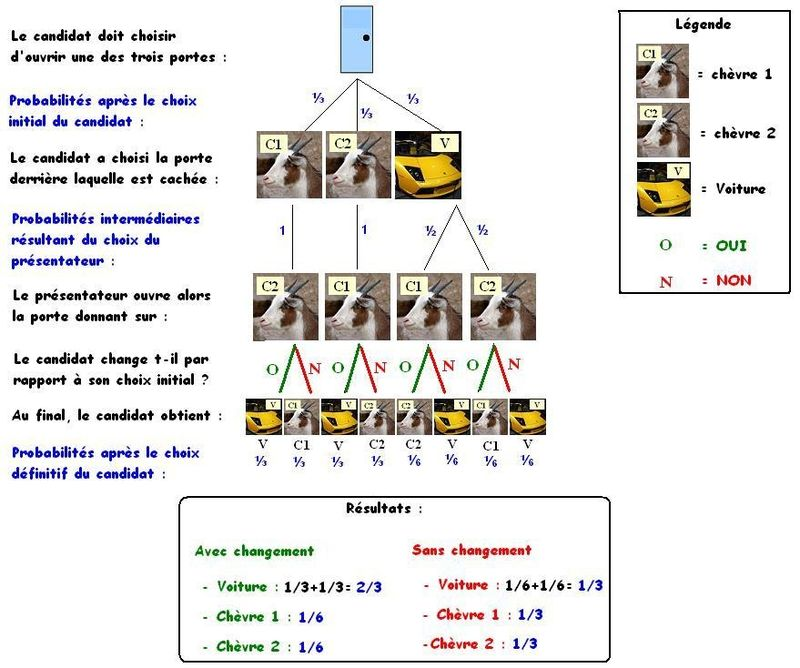
\includegraphics[width=1.1\textwidth]{images/SolutionMontyHall.JPG}
    
\end{figure}

\textit{Arbre de probabilité ; Analyse de la situation ; Paradoxe mathématique ; Fonction d'onde ; Choix; Réalité pas toujours aussi simple qu'il n'y paraît.}
\end{cor}


\begin{cor}
Pour cet exercice, il est très important de se rendre compte que, lorsque le géant tire l'élastique, c'est l'ensemble de l'élastique qui s'allonge (dont la partie derrière l'escargot) \textit{On peut parler de la loi de Hook}. Il est alors utile de considérer le pourcentage de progression de l'escargot. Cette quantité ne varie pas lorsque que le géant agit.

On a donc à la $n$-ième étape une longueur de l'élastique de $n*l$. L'augmentation du pourcentage de progression de l'escargot à chaque étape est donc de $v/(nl)$. Le pourcentage total à la $n$-ième étape s'obtient en sommant : $p_n = \sum v/(nl)$, et cette somme diverge ! \textit{Pour le démontrer, on peut se servir du fait que $S_{2n} - S_n > 1/2$.}

Pour estimer le temps de parcours, il faut calculer $n$ tel que : $p_n = 1$. Pour ce faire, il faut expliquer que $p_n \sim (v/l) \ln(n)$. Le temps nécessaire est donc d'environ $\exp(l/v)$ (c'est énorme) !\newline


\textit{Cet exercice permet d'introduire plein de notions sur les suites et de manière de les voir; Notion de convergence ; Somme (in)finie.}
\end{cor}


\begin{cor}
Très classique, il s'agit d'une démonstration par disjonction de cas : on commence par regarde tous les solides réguliers qu'on forme avec un triangle pour face, puis un carré, puis un pentagone, puis un hexagone, et enfin on élimine la possibilité d'avoir des face formées avec des polygones à plus de côtés. On va assembler plusieurs éditions d'un polygone régulier à un sommet pour savoir s'il est possible de créer un solide grâce à cela.

Sur un même sommet, doivent se rejoindre au moins 3 faces :
\begin{enumerate}
\item \textbf{Avec 3 triangles équilatéraux à chaque sommet, on obtient un tétraèdre.}
\item \textbf{Avec 4, on obtient un octaèdre.}
\item \textbf{Avec 5, on obtient un icosaèdre}
\item On ne peut mettre 6 triangles équilatéraux à un sommet car la somme des angles fait alors $2\pi$, l'objet obtenu est plat.
\item \textbf{Avec 3 carrés, on obtient un cube.}
\item Avec 4 carrés, on a encore un angle de $2\pi$, donc pas de solide.
\item \textbf{Avec 3 pentagones, on obtient un dodécaèdre.}
\item Avec 4 pentagones, l'angle dépasse $2\pi$, le solide n'est pas constructible.
\item Avec 3 hexagones (ou un polygone à plus de côté), l'angle dépasse les $2\pi$, donc plus aucun solide n'est constructible.
\end{enumerate}

On a obtenu les 5 solides de Platon.\newline

\begin{figure}[h!]
	\centering
    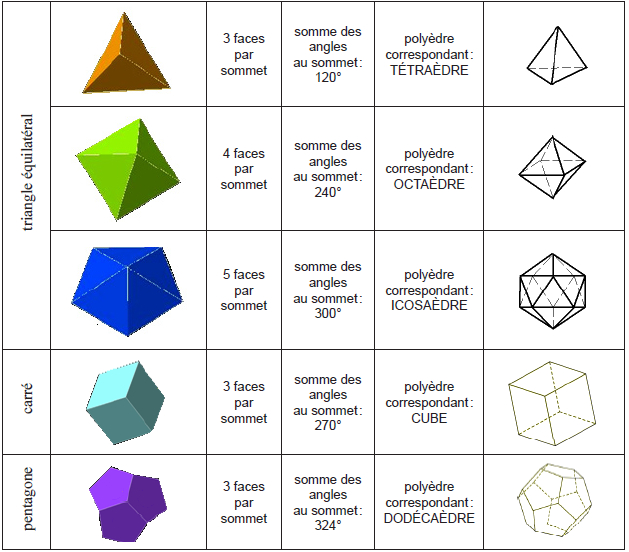
\includegraphics[width=0.8\textwidth]{images/PolyedreSolution.jpg}  
\end{figure}

\textit{Raisonnement en 3 dimensions; Introducion à la disjnction des cas; Culture mathématique; Raisonnement classique; Logique.}

\end{cor}


\end{document}  